\section{ОБЗОР ЛИТЕРАТУРЫ}
\label{sec:domain}

% добавить о чем будет говориться в дипломе, какие темы будут расмотрены, что будет реальизовано

\subsection{Метод калибровки магнетометра}
% https://www.ncbi.nlm.nih.gov/pmc/articles/PMC8401862/
% https://teslabs.com/articles/magnetometer-calibration/
Калибровка магнетометра -- это критически важный этап для обеспечения точности измерений магнитного поля. 
Суть этого процесса заключается в выявлении и компенсации различных видов погрешностей, которые могут 
влиять на получаемые данные. Эти погрешности делятся на две категории: статические и динамические смещения.
Статические смещения постоянны во времени и обусловлены особенностями производства датчиков, например,
неидеальностью материалов, неточностью монтажа. Среди таких помех существуют: 
\begin{itemize}
    \item смещение нуля: отклонение измеряемого значения от истинного нуля;
    \item масштабный коэффициент: неравномерность чувствительности датчика по различным осям;
    \item ненулевая ортогональность: неидеальность взаимного расположения осей чувствительности датчика.
\end{itemize}

Динамические смещения переменны во времени и вызваны внешними факторами окружающей среды, например, магнитными помехами
вызванные ближайшими электронными устройствами и металлическими предметами, 
а также температурные изменения, к которым может быть чувствителен датчик.

Почти все методы калибровки используют упрощенную модель измерения трехосного магнетометра:

\begin{equation}
    \label{eq:domain:magnetModel}
    y = Tm+h+e,
  \end{equation}
  \begin{explanationx}
    \item[где] $h$ -- жесткие смещения, то есть смещения вызванные материалами, которые вызывают смещения, прикрепленные к системе координат, такие материалы генерируют собственное  постоянное магнитное поле;
    \item      $T$ -- мягкие смещение (представляет собой матрицу 3x3) -- смещения, вызванные наличием ферромагнитных материалов вблизи датчика (не генерируют магнитные поля, только искажают);
    \item      $e$ -- случайный шум, вызванные особенностями механической и электрической архитектуры датчика, считается, что это последовательность белого шума;
    \item      $m$ -- истинное магнитное поле;
    \item      $y$ -- искаженное магнитное поле.
  \end{explanationx}

Используемый в дипломном проекте метод калибровки магнетометра, называемый <<MAG.I.C.AL>>, предполагает, что данные измерений магнитометра
лежат на эллипсоиде согласно модели измерений, то есть набор векторов, представляющий измерения магнетометра по трём осям, 
имеет вид на трехмерной плоскости в виде эллипсоида ~\cite{magical}. %%TODO: add link to equitation %%. 

%TODO: поправить формулу%
Для алгоритма требуется проинициализировать вектора магнитного поля:

\begin{equation}
    \label{eq:domain:initMK}
    m_{k} = \frac{y_{k}}{\left|y_{k}\right|}, k=1,2,3,\dots ,K,
  \end{equation}
  \begin{explanationx}
    \item[где] $K$ -- количество измерений.
  \end{explanationx}

Алгоритм использует другую форму модели измерений записанную как:

\begin{equation}
    \label{eq:domain:updatedMagnetModel}
    Y = LG+E,
  \end{equation}
  \vspace{-1ex}
\begin{equation}
    \label{eq:domain:Y}
    Y = \begin{bmatrix}
        y_{1} & y_{2} & \dots & y_{K}
        \end{bmatrix}
        \text{,}
\end{equation}
\vspace{-1ex}
\begin{equation}
    \label{eq:domain:L}
    L = \begin{bmatrix}
        T & h
        \end{bmatrix}
        \text{,}
  \end{equation}
  \vspace{-1ex}
\begin{equation}
    \label{eq:domain:G}
    G = \begin{bmatrix}
        m_{1} & m_{2} & \dots & m_{K} \\
        1 & 1 & \dots & 1
        \end{bmatrix}
        \text{,}
        \vspace{-0.1ex}
  \end{equation}
\begin{equation}
    \label{eq:domain:E}
    E = \begin{bmatrix}
            e_{1} & e_{2} & \dots & e_{K}
        \end{bmatrix}
        \text{,}
  \end{equation}

$L$ ищется при помощи метода наименьших квадратов, используя формулу:

\begin{equation}
    \label{eq:domain:findL}
    L=YG^{T}(GG^{T})^{-1}
  \end{equation}

По полученным параметрам $T$ и $h$ извлеченных из $L$, обновим вектор магнитного поля $m_{k}$:

\begin{equation}
    \label{eq:domain:updateMk}
    m_{k}=\frac{m_{k}^{'}}{\left|m_{k}^{'}\right|}
  \end{equation}
  \begin{explanationx}
    \item[где] $m_{k}^{'}$ найдено из формулы:
  \end{explanationx}

\begin{equation}
    \label{eq:domain:findNewMk}
    m_{k}^{'}=T^{-1} \cdot (y_{k}-h)
  \end{equation}

Далее вычисленный вектор оценивается при помощи функции:

\begin{equation}
    \label{eq:domain:findError}
    J(T, h) = \sum_{k=1}^{K}(|m_{k}^{'}|^{2}-1)^{2}
  \end{equation}

Если оценка не достигла минимального значения, то $G$ обновляется вычисленным вектором $m~k$ и снова вычисляется $T$ и $h$.
Обобщенно алгоритм можно представить так:
% TODO:Добавить ссылки на формулы %.
% TODO:Дизобразить в виде блок схемы%.
\begin{enumerate_num}
    \item Инициализация $m_{k}$ по формуле \ref{eq:domain:initMK}.
    \item Расчет $L$ по формуле \ref{eq:domain:findL}.
    \item Извлечение $T$, $h$ из $L$, формула \ref{eq:domain:L}.
    \item Обновление вектора $m_{k}$ из формулы \ref{eq:domain:updateMk}.
    \item Оценка полученного вектора $m_{k}$, по формуле \ref{eq:domain:findError}.
    \item Повтор шага 2-5.
\end{enumerate_num}

\subsubsection{Сравнение актуальных алгоритмов калибровки магнетометра}

Помимо выбранного алгоритма калибровки магнетометра существуют также другие способы вычислить параметры $T$ и $h$. 
В статье~\cite{mag_calib_cmp}~ приводится сравнение известных алгоритмов по их точности, надежности и среднему времени выполнения, степени простоты.
Параметр точности определяется как среднее значение отклонений (разница полученных параметров $h$ и $T$ от истинных $h$ и $T$) 
для всех $N$ тестов (больше  -- лучше). Средняя частота выполнения определяется как среднее значение частоты  выполнения алгоритма (больше  -- лучше).
Надежность определяется как процент наборов данных, для которых каждый алгоритм успешно нашел значимое решение (больше  -- лучше).

Все величины для простоты понимания сравнения алгоритмов приведены к безразмерным величинам, которые нормализованны от нуля до единицы.
Некоторые алгоритмы названы первой фамилией, того кто придумал и описал алгоритм.
\begin{table}[ht]
    \caption{Сравнение алгоритмов калибровки магнетометра}
    \label{table:domain:magnet_calib_comp}
    \begin{tabular}{| >{\centering}m{0.25\textwidth}
                    | >{\centering}m{0.2\textwidth}
                    | >{\centering}m{0.2\textwidth}
                    | >{\centering\arraybackslash}m{0.25\textwidth}|}
        \hline
        \centering Название & \centering Точность & \centering Надежность & \centering\arraybackslash Частота выполнения \\
        \hline

        TWOSTEP & 
        0 & 
        0.916 & 
        1 
        \\
        \hline

        Crassidis & 
        0.014 & 
        1 & 
        0.104 
        \\
        \hline

        Dorveaux & 
        0.974 & 
        1 & 
        0.028 
        \\
        \hline

        Vasconcelos & 
        0.983 & 
        0.996 & 
        0 
        \\
        \hline

        Ali & 
        0.978 & 
        0.988 & 
        0.00002
        \\
        \hline

        Wu and Shi & 
        1 & 
        0.872 & 
        0.00033 
        \\
        \hline

        MAG.I.C.AL & 
        0.983 & 
        1 & 
        0.064 
        \\
        \hline
    \end{tabular}
\end{table}

Исходя из полученного сравнения алгоритм <<MAG.I.C.AL>> обладает лучшей оценкой.

\subsection{Метод калибровки акселерометра и гироскопа}

На измерения гироскопа и акселерометра влияют такие параметры как чувствительность датчика и смещение относительно нуля.
На такие параметры в датчике обычно влияет температура.
Для описания модели измерений можно воспользоваться формулой \ref{eq:domain:magnetModel}, которую можно преобразовать до вида:

\begin{equation}
    \label{eq:domain:accModel}
    y = Xm+e,
  \end{equation}
  \begin{explanationx}
    \item[где] $X$ -- матрица состоящая из $T$ и $h$;
  \end{explanationx}

В формуле $T$ описывает параметр чувствительности, а параметр $h$ смещение относительно нуля.
Для калибровки гироскопа в разрабатываемом модуле не предусмотрен поиск параметра $T$ в силу того, 
что нужно разрабатывать отдельный калибровочный стенд способный вращать устройство с определенной 
угловой скоростью относительно каждой оси трехмерной системы координат. Но описанный ниже алгоритм подходит для двух типов датчиков, 
только вместо ускорения свободного падения относительно каждой оси нужно заменить на угловую скорость.

Для алгоритма потребуются начальные входные данные от неоткалиброванного устройства в шести положениях относительно датчика.
\begin{enumerate_num}
    \item Положение осью $X$ вниз.
    \item Положение осью $X$ вверх.
    \item Положение осью $Y$ вниз.
    \item Положение осью $Y$ вверх.
    \item Положение осью $Z$ вниз.
    \item Положение осью $Z$ вверх.
\end{enumerate_num}

Для каждого положения определим эталонный вектор свободного ускорения падения $Y$, например для положения осью $X$ вверх, вектор $Y$ имеет вид:

\begin{equation}
    \label{eq:domain:Yxup}
    Y_{xвверх} = \begin{bmatrix}
            1 & 0 & 0
        \end{bmatrix}
        \text{,}
  \end{equation}

Для положения осью Z вниз, эталонный вектор будет иметь вид:

\begin{equation}
    \label{eq:domain:Yzdown}
    Y_{zвниз} = \begin{bmatrix}
            0 & 0 & -1
        \end{bmatrix}
        \text{,}
  \end{equation}

Также для каждого положения нужно получить набор неоткалиброванных данных. 
К вектору неоткалиброванных данных нужно добавить еще один четвертый элемент 1, теперь вектор входных данных имеет вид:

\begin{equation}
    \label{eq:domain:XL_meas}
    m = \begin{bmatrix}
            m_{x} & m_{y} & m_{z} & 1
        \end{bmatrix}
        \text{,}
  \end{equation}

Далее нужно сформировать полный набор данных, как эталонных так и выходных, матрицы будут иметь вид:

\begin{equation}
    \label{eq:domain:XL_Y_dataset}
    Y = \begin{bmatrix}
            Y_{xвниз} \\ Y_{xвверх} \\ \dots \\ Y_{zвверх}
        \end{bmatrix}
        \text{,}
  \end{equation}


\begin{equation}
    \label{eq:domain:XL_M_dataset}
    m = \begin{bmatrix}
            m_{xвниз} \\ m_{xвверх} \\ \dots \\ m_{zвверх}
        \end{bmatrix}
        \text{,}
  \end{equation}

Следующим шагом используя метод наименьших квадратов можно определить калибровочные параметры \cite{accelerometer}:

\begin{equation}
    \label{eq:domain:XL_CALIB}
    X = \left[m^T \cdot m\right]^{-1}\cdot m^T \cdot Y
  \end{equation}

Данный алгоритм достаточно популярен за счет простоты математических расчетов, недостатком можно выделить то, что 
для алгоритма требуется большой набор данных состоящий из набора векторов для каждой оси, в микроконтроллерах ограниченных небольшим 
количеством памяти требуется оптимизировать алгоритм. 

\subsection{Фильтр Маджвика}

Чтобы оценить ориентацию тела в пространстве, нужно для начала выбрать какие-то параметры, 
которые в совокупности однозначно определяют эту ориентацию, т.е. по сути ориентацию связанной 
системы координат $xyz$ относительно условно неподвижной системы -- например, географической системы NED (North, East, Down). 
Затем нужно составить кинематические уравнения, т.е. выразить скорость изменения этих параметров через угловую скорость от 
гироскопов. Наконец, нужно ввести в расчёт векторные измерения от акселерометра.

Одним из способов представить ориентацию тела в пространстве является квантерион, который используется фильтром Маджвика в расчетах.
Это четырехмерное комплексное число $q=q_{0}+q_{1}i+q_{2}j+q_{3}k$, которое может быть использовано 
для представления ориентации тела в трехмерном пространстве.
Описать связь квантериона с теоремой Эйлера можно через преобразования квантериона в углы Эйлера: 

%https://habr.com/ru/articles/255661/%
%https://habrastorage.org/r/w1560/files/b65/424/f94/b65424f943e5432185bdc29631cd5d37.png%
\begin{equation}
    \label{eq:domain:QtoPhi}
    \phi = \arctan{\frac{2q_{3}q_{4}-2q_{1}q_{2}}{2q_{1}^{2} + 2q_{4}^{2}-1}}
    \end{equation}
\begin{explanationx}
    \item[где] $\phi$  -- это курс, поворот вокруг оси $X$ в системе углов Эйлера.
    \end{explanationx} 

    \begin{equation}
        \label{eq:domain:QtoTheta}
        \theta = \sin^{-1}{2q_{2}q_{4}+2q_{1}q_{3}}
    \end{equation}
    \begin{explanationx}
        \item[где] $\theta$  -- это тангаж, поворот вокруг оси $Y$ в системе углов Эйлера.
    \end{explanationx} 

\begin{equation}
    \label{eq:domain:QtoPsi}
    \psi = \arctan{\frac{2q_{2}q_{3}-2q_{1}q_{4}}{2q_{1}^{2} + 2q_{2}^{2}-1}}
    \end{equation}
    \begin{explanationx}
        \item[где] $\psi$  -- это курс, поворот вокруг оси $Z$ в системе углов Эйлера.
        \end{explanationx}
        
Целью фильтра Мэджвика и похожих фильтров, является компенсация дрейфа гироскопа по времени и по температуре.
Используя квантерионы, которые позволяют представить данные акселерометра и магнетометра пригодные для решения задачи оптимизации 
методом градиентного спуска для того чтобы выявить погрешность измерений гироскопа связанных с дрейфом. Это эффективная в 
вычислительном отношении альтернатива фильтру Калмана, что делает ее подходящей для приложений реального времени во встроенных 
системах с ограниченными ресурсами. 

Преимуществами данного фильтра являются:

\begin{itemize}
    \item дешевизна по вычислительным ресурсам -- 277 простых арифметических операций каждое обновление фильтра;
    \item эффективность при низких частотах дискретизации (например 10 Гц).
\end{itemize}

Недостатком фильтра является множество параметров к которым он восприимчив, поэтому его настройка должна быть очень тщательная.
% TODO: add bibliography link to the madgwick explanation

\begin{figure}[ht]
    \centering
    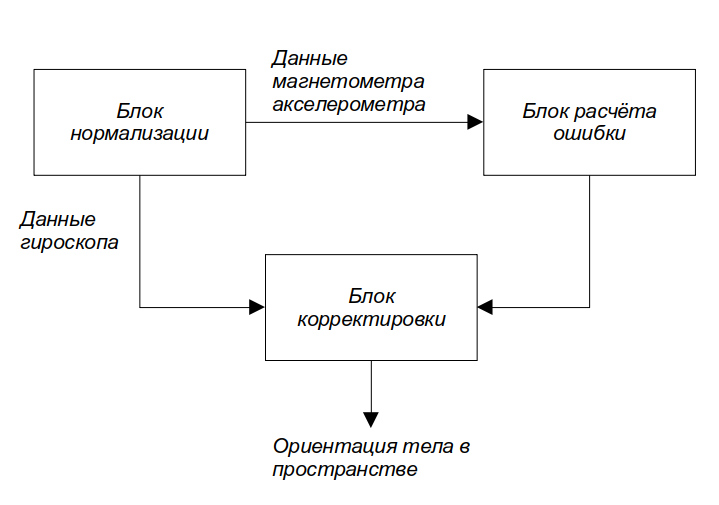
\includegraphics[width=1.0\linewidth]{madgwick}
    \caption{Блок-схема фильтра Мэджвика}
    \label{pic::domain::madgwick}
\end{figure}


Фильтр состоит из нескольких блоков представленных на рисунке~\ref{pic::domain::madgwick}.
Первый блок это прием данных и их нормализация для обеспечения одинакового 
масштаба поступаемых с датчиков данных.
Второй блок вычисляет ошибку между прогнозируемыми (на основе предполагаемой ориентации) и поступающими данными, 
эта ошибка используется следующим блоком.
Следующий, ключевой, в фильтре блок -- это реализация градиентного спуска, который 
использует итерационный процесс для минимизации ошибки между прогнозируемыми и 
измеренными значениями датчика. Алгоритм вычисляет градиент функции ошибок и корректирует
предполагаемую ориентацию (представленную в виде кватерниона) для достижения минимальной ошибки.
Все это вместе компенсирует дрейф гироскопа, который накапливается со временем.

\subsection{Метод расчета азимута с учетом наклона устройства}

После калибровки данных, полученных от магнетометра, следуют расчеты азимута в сторону сервера.
Для прибора который находится в свободном положении это может быть проблемой с учетом того, что
он может быть наклонен и угол проекции вектора измерений магнетометра может не совпасть с настоящим азимутом.
Для этого требуется поправка азимута с учетом наклона устройства. Принцип заключается в использовании 
поворотной матрицы, которая поворачивает ось измерений согласно наклону устройства. Наклон устройства 
считывается с датчиков акселерометра и гироскопа.

Для расчета азимута потребуется только две оси магнетометра $x$,$y$, ось $z$ в расчетах будет избыточной.
Чтобы представить азимут в радианах нужно воспользоваться формулой:

\begin{equation}
    \label{eq:domain:rawAzimuth}
    azimuth = \arctan\left(\frac{Hx}{Hy}\right),
  \end{equation}
  \begin{explanationx}
    \item[где] $H_x$  -- измерения магнетометра по оси $x$;
    \item $H_y$  -- измерения магнетометра по оси $y$.
  \end{explanationx}

Для поворота системы координат можно использовать как квантерионы, так и углы Эйлера.
Если представлять поворот стационарной (неподвижную) системы координат в наклоненную систему, то
необходимо повернуть ось X на угол крена ($\theta$)~, а ось Y на угол тангажа ($\phi$).
Представить стационарную систему координат в наклоненную систему можно при помощи матрицы поворота --
матрица $C$ размера 3×3, на которую нужно умножить любой вектор в связанной системе координат, 
чтобы получить тот же вектор в географической системе.

Поворотная матрица оси X выглядит следующим образом: \\

\begin{equation}
    \label{eq:domain:rotateXmat}
    С_{X} = \begin{bmatrix} 1 & 0 & 0 \\ 
        0 & \cos{\theta} & -\sin{\theta} \\ 
        0 & -\sin{\theta} & \cos{\theta} \\ 
        \end{bmatrix}
    \end{equation}

Для поворота оси Y матрица будет выглядеть так:\\

\begin{equation}
    \label{eq:domain:rotatYmat}
    C_Y = \begin{bmatrix} \cos{\theta} & 0 & -\sin{\theta} \\ 
        0 & 1 & 0 \\ 
        \sin{\phi} & 0 & \cos{\phi} \\ 
    \end{bmatrix}
    \end{equation} 

Влияние поворота устройства на поворот его стационарной систему координат,
можно записать следующим образом:

\begin{equation}
    \label{eq:domain:magnetTilt}
    \begin{bmatrix} x^{'} \\ y^{'} \\ z^{'} \\ \end{bmatrix} = 
            С_X \cdot С_Y \cdot \begin{bmatrix} x \\ y \\ z \\ \end{bmatrix}
    \end{equation} 

\begin{equation}
    \label{eq:domain:magnetTiltExtendet}
    \begin{bmatrix} x^{'} \\ y^{'} \\ z^{'} \\ \end{bmatrix} = 
    \begin{bmatrix} \cos{\phi} & 0 & -\sin{\phi} \\ 
        \sin{\phi}sin{\theta} & \cos{\theta} & \sin{\theta}cos{\phi} \\ 
        \cos{\theta}sin{\phi} & -\sin{\theta} & \cos{\theta}cos{\phi} \\ 
    \end{bmatrix}
    \cdot
    \begin{bmatrix} x \\ y \\ z \\ \end{bmatrix}
    \end{equation} 

Магнитный датчик измеряет компоненты $x^{'}$, $y^{'}$, $z^{'}$  магнитного вектора Земли. 
Для определения азимута эти значения должны быть преобразованы в стационарную систему координат.
Это преобразование выполняется с использованием инвертированной матрицы вращения:

\begin{equation}
    \label{eq:domain:invMagnetTilt}
    \begin{bmatrix} x \\ y \\ z \\ \end{bmatrix} = 
    \begin{bmatrix} \cos{\phi} & \sin{\phi}sin{\theta} & \cos{\theta}sin{\phi} \\ 
        0 & \cos{\theta} & -\sin{\theta} \\ 
        -\sin{\phi} & \sin{\theta}cos{\phi}& \cos{\theta}cos{\phi} \\ 
    \end{bmatrix}
    \cdot
    \begin{bmatrix} x^{'} \\ y^{'} \\ z^{'} \\ \end{bmatrix}
    \end{equation} 

Так как координата $z$ не используется в расчетах можно упростить формулу до вида:

\begin{equation}
    \label{eq:domain:xMagnetTilt}
    x = x'\cos{\phi}+y'\sin{\theta}\sin{\phi}+z'\cos{\theta}\sin{\phi}
    \end{equation} 

\begin{equation}
    \label{eq:domain:yMagnetTilt}
    y = y'\cos{\theta}+z'\sin{\theta}
    \end{equation} 

Углы $\phi$, $\theta$ могут быть получены исходя из данных полученных от гироскопа и акселерометра.

% https://www.ncei.noaa.gov/products/world-magnetic-model
\begin{figure}[ht]
    \centering
    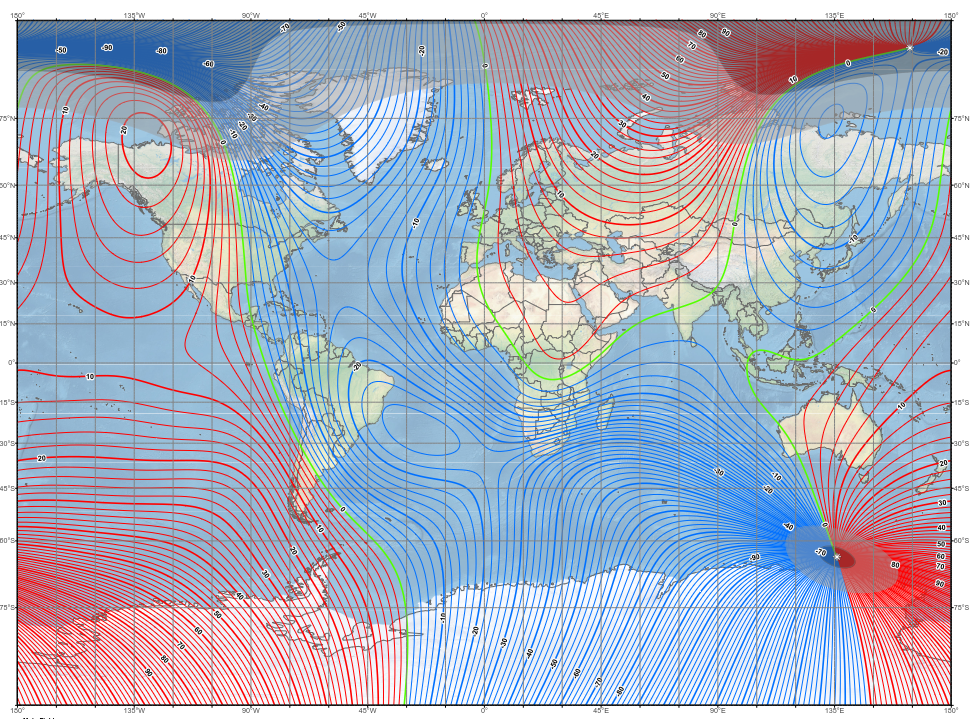
\includegraphics[width=1.0\linewidth]{wmm}
    \caption{Магнитная модель Земли \cite{magnet_declination}}
    \label{pic:domain:wmm}
\end{figure}

После перечета координат x, y к стационарной системе координат, можно рассчитать азимут, 
а также чтобы преобразовать полученный азимут как угол отклонения часовой стрелки нужно 
учитывать знаки $x$ и $y$:
\begin{equation}
    azimuth =
    \begin{cases}
      \pi - \arctan\left(\frac{y}{x}\right) \text{, x<0}\\      
      - \arctan\left(\frac{y}{x}\right) \text{, x>0, y<0} \\
      2\pi - \arctan\left(\frac{y}{x}\right) \text{, x>0, y>0} \\
      90 \text{, x=0, y<0} \\
      270 \text{, x=0, y>0}
    \end{cases}
\end{equation}

Также на компас действует магнитное наклонение Земли -- угол, на который отклоняется стрелка под действием 
магнитного поля Земли в вертикальной плоскости. Для уточнения азимута нужно использовать магнитную модель Земли
и текущие координаты.
Достоверная модель показана на рисунке \ref{pic:domain:wmm}.

\subsection{БИХ-фильтр}
%http://www.dsplib.ru/content/filters/butterex/butterex.html
БИХ фильтр  -- это цифровой фильтр с
бесконечной во времени импульсной характеристикой, 
то есть имеет очень большое или бесконечное число коэффициентов. БИХ фильтры также 
называют рекурсивными в связи с тем, что при их
реализации используются обратные связи (сигнал с выхода фильтра через элементы задержки 
поступает на фильтр и вносит изменения сам в себя). 
Передаточная функция БИХ-фильтра имеет дробно-рациональный вид. Основные известные БИХ-фильтры: 
фильтр Чебышева, Баттерворта, Калмана, Бесселя и т.д.
Каноническая структурная схема фильтра представлена на рисунке \ref{pic:domain:iic}, разностное уравнение БИХ-фильтра:

\begin{equation}
    \label{eq:domain:eqIIC}
    y(n) = \sum_{k=0}^{N}b_{k}x(n-k) - \sum_{k=1}^{M}a_{k}y(n-k)
    \end{equation}
    \begin{explanationx}
        \item[где] $a_{k}$, $b_{k}$  -- это коэффициенты фильтра.
      \end{explanationx} 

      \begin{figure}[ht]
        \centering
        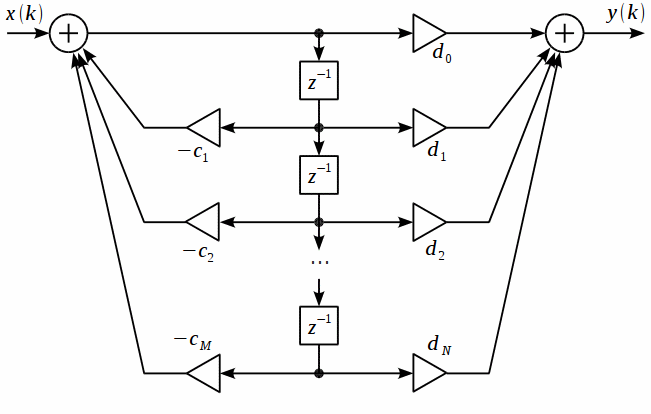
\includegraphics[width=1.0\linewidth]{iic}
        \caption{Каноническая структурная схема БИХ фильтра}
        \label{pic:domain:iic}
    \end{figure}

Из уравнения видно, что выходной сигнал фильтра за счет обратных связей влияет сам на себя. 
Также уравнение можно представить как свертку входного сигнала и импульсной характеристики фильтра $h(n)$:

\begin{equation}
    \label{eq:domain:convolution}
    y(n) = h(n) \ast  x(n)
    \end{equation}

Уравнение \ref{eq:domain:convolution} при помощи Z преобразования удобно представить в виде произведения Z-образов входной последовательности X(z) и передаточной функции H(z):

\begin{equation}
    \label{eq:domain:Zconvolution}
    Y(z) = H(z)X(z)
    \end{equation}

Для расчета коэффициентов фильтра удобно использовать аналоговый прототип \cite{dsp} для получения передаточной характеристики. 
Это достаточно известный и широко используемый метод, для расчетов потребуется наличие нескольких параметров:

\begin{itemize}
    \item $\omega_{p}$  -- нормированная частота среза;
    \item $\omega_{s}$  -- нормированная частота заграждения;
    \item $R_{p}$  -- неравномерность в полосе пропускания;
    \item $R_{s}$  -- уровень подавления в полосе заграждения.
\end{itemize}

В дипломном проектировании используется фильтр нижних частот (ФНЧ) на основе фильтр Баттерворта, 
который был выбран за счет того что имеет максимально плоскую амплитудно-частотную характеристику
(АЧХ) в полосе пропускания и монотонно возрастающее затухание в полосе задерживания.

Первое, что нужно рассчитать это искажение частот при переходе от аналогового фильтра к цифровому, поскольку в дальнейшем для
расчета фильтра будет использовано билинейное преобразование (преобразование передаточной непрерывной формы $H(s)$ в дискретную передаточную функцию $H(z)$), 
неравномерность в полосе пропускания и уровень подавления в полосе 
заграждения не меняются при переходе от аналогового фильтра к цифровому. 
Искажение рассчитывается формулой:

\begin{equation}
    \label{eq:domain:Omega}
    \Omega=\frac{2}{T}\tan{\frac{\omega}{2}}
    \end{equation}
    \begin{explanationx}
        \item[где] $T$  -- интервал дискретизации;
        \item      $\Omega$  -- пересчитанная шкала частот для аналогового фильтра;
        \item      $\omega$  -- шкала частот цифрового фильтра.
      \end{explanationx} 

Далее нужно рассчитать порядок ФНЧ Баттерворта:

\begin{equation}
    \label{eq:domain:NIIC}
    N=\frac{log{\frac{\sqrt{10^{R_{s}/10}-1}}
                     {\sqrt{10^{R_{p}/10}-1}}}}
           {\log{\frac{\Omega_{s}}
                      {\Omega_{p}}}}
    \end{equation}


Порядок округляется до ближайшего целого и далее вычисляется передаточная характеристика:

\begin{equation}
    \label{eq:domain:Hz}
    H(z) = \frac{1}
                {\epsilon_{p} (s + \alpha )^r \cdot \prod_{n=1}^{L} (s^{2} + 2 \alpha \sin{ \theta_{n} s + \alpha^{2}})}
    \end{equation}

\begin{equation}
        \label{eq:domain:whereN}
        N=2 \cdot L+r
        \end{equation}

\begin{equation}
        \label{eq:domain:whereAlpha}
        \alpha=\frac{1}
                    {\sqrt[N]{\sqrt{10^{R_{p}/10}-1}}}
        \end{equation}

\begin{equation}
        \label{eq:domain:whereTheta}
        \theta_{n}=\frac{2\cdot n - 1}
                        {2\cdot N} \cdot \pi
        \end{equation}

\begin{equation}
        \label{eq:domain:whereS}
        s=\frac{2}
                {T\cdot \Omega_{p}} \cdot \frac{1-z^{-1}}
                                                {1+z^{-1}}
        \end{equation}

Данное уравнение необходимо упростить до вида:

\begin{equation}
    \label{eq:domain:canonHz}
    H(z)=\frac{\sum_{i=0}^{N}b_{i}\cdot z^{-i}}{1+\sum_{k=1}^{N-1}\cdot a_{k}z^{-k}}
    \end{equation}

Полученные коэффициенты $a_{m}$, $b_{i}$ являются искомыми коэффициентами ФНЧ. % ссылка на формулу фильтра

% \subsection{Расчет азимута между двумя объектами}

% Для расчетов угла объекта относительно другого объекта используется расчет с использованием
% текущей широты одного объекта, и координат другого, представить азимут цели можно при помощи формулы:

% \begin{equation}
%     \label{eq:domain:baring}
%     \theta=\arctan{\frac{\sin{\lambda_2 - \lambda_1} \cdot \cos{\phi_{2}}}{\cos{\phi_{1}} \cdot \sin{\phi_{2}} - \sin{\phi_{1}} \cdot \cos{\phi_{2}} \cdot \cos{\lambda_2 - \lambda_1}}}
%     \end{equation}

%     \begin{explanationx}
%         \item[где] $\phi_1$  -- широта объекта 1;
%         \item      $\lambda_1$  -- долгота объекта 1;
%         \item      $\phi_2$  -- широта объекта 2;
%         \item      $\lambda_2$  -- долгота объекта 2.
%       \end{explanationx} 
